\documentclass[../main.tex]{subfiles}
\graphicspath{{\subfix{../images/}}}
\begin{document}
\section*{Term 1 Week 2}
    \begin{enumerate}
    \item 
    We need to find \(\frac{d\theta}{dt}\) when y=10.\\
    \(\frac{dy}{dt}=3\)\\
    
    \( \frac{d\theta}{dt}=\frac{dy}{dt}\times \frac{d\theta}{dy}\)\\
    
    Use \(\tan{\theta}=\frac{y}{25}\), which is the same as \(y=25 \tan{\theta}\)\\

    \(\frac{dy}{d\theta}=25\sec^2{\theta}=\frac{25}{\cos^2{\theta}}\)\\

    \(\frac{d\theta}{dt}=3\times \frac{\cos^2{\theta}}{25}\)\\

    When y=10, \(\tan{\theta}=\frac{10}{25}\)\\

    \(\theta=\tan^-1{(\frac{10}{25})}=0.38\)\\

    Therefore, \(\frac{d\theta}{dt}=\frac{3\cos^2{0.38}}{25}=0.103\)rad/sec.\\

    \item 
    Use similar shapes:\\
    \begin{figure}[H]
        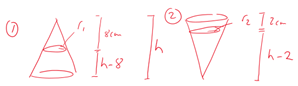
\includegraphics{images/t1w2q2_a.png}
    \end{figure}
    \(h-2 : r_2 = 8 : r_1\)\\
    \(\frac{h-2}{r_2}=\frac{8}{r_1}\)\\
    \(r_1=\frac{8r_2}{h-2}\)\\

    \(h:r=8:r_1\)\\
    \(\frac{h}{r}=\frac{8}{r_1}\)\\
    \(r=\frac{r_1 h}{8}\)\\

    Volume = \(\frac{1}{3}\pi r^2 h\)\\

    From diagram 1:\\
    \(V=\frac{1}{3}\pi r^2 h-\frac{1}{3}\pi r_1^2 \times 8\)\\

    \(V=\frac{1}{3}\pi (\frac{r_1 h}{8})^2 h-\frac{1}{3}\pi r_1^2 \times 8\)\\

    \(V=\frac{1}{3}\pi r_1^2(\frac{h^3}{64}-8)\)\\

    From diagram 2:\\
    \(V=\frac{1}{3}\pi r_2^2 (h-2)\)\\

    Substituting \(r_1 =\frac{8r_2}{h-2} \) we can then equate our volume equations.\\
    \(\frac{1}{3}\pi (\frac{8r_2}{h-2})^2(\frac{h^3}{64}-8)=\frac{1}{3}\pi r_2^2 (h-2)\)\\

    \(\frac{64}{(h-2)^2}(\frac{h^3}{64}-8)=h-2\)\\

    \(h^3-512=(h-2)^3\)\\

    \(h^3=512=h^3-6h^2+12h-8\)\\

    \(6h^2-12h-504=0\)\\

    \(h=10.2195, -8.2195\)\\

    Therefore, the height is 10.2cm.\\

    \item 
    Scale up each factor so they have \(x^5\) in the numerator.\\

    \(\frac{x}{1+x^2}\times \frac{x^4}{x^4}+\frac{x^2}{1+x^4}\times \frac{x^3}{x^3}+\frac{x^3}{1+x}\times \frac{x^2}{x^2}+\frac{x^4}{1+x^3}\times \frac{x}{x}\)\\

    \(=\frac{x^5}{x^4+x^6}+\frac{x^5}{x^3+x^7}+\frac{x^5}{x^2+x^3}+\frac{x^5}{x+x^4}\)\\

    Now, consider that if \(x^5=1\), then \(x^6=x\) and \(x^7=x^2\), so we can rewrite the expression as:\\

    \(\frac{1}{x^4+x}+\frac{1}{x^3+x^2}+\frac{1}{x^2+x^3}+\frac{1}{x+x^4}=\frac{2}{x+x^4}+\frac{2}{x^2+x^3}\)\\

    Combining into one fraction with a common denominator:\\
    \(\frac{2}{x+x^4} \times \frac{x^2+x^3}{x^2+x^3}+\frac{2}{x^2+x^3}\times \frac{x+x^4}{x+x^4}=\frac{2x^2+2x^3+2x+2x^4}{(x+x^4)(x^2+x^3)}=\frac{2(x+x^2+x^3+x^4)}{x^3+x^4+x^6+x^7}\)\\

    Using the same trick as above, we can rewrite it as:\\
    \(\frac{2(x+x^2+x^3+x^4)}{x+x^2+x^3+x^4}=2\)
    \end{enumerate}
\end{document}
